% Note to reader: lines beginning with the '%' character are
% 'comments' to you, the human reader of this code, and are 
% ignored by the LaTeX compiler.

%%%%%%%%%%%%%%%%%%%%%%%%%%%%%%%%%%%%%%%%%%%%%%%%%%%%%%%%%%%%%%%%%%
% = Sample template for MIT Junior Lab Student Written Summaries =
% Available from 
%    http://web.mit.edu/8.13/www/Samplepaper/sample-paper.tex
%
% Last Updated July 23, 2014
%
% Adapted from the American Physical Societies REVTeK-4.1 Pages
%    at http://publish.aps.org
%
% ADVICE TO STUDENTS: Each time you write a paper, start with this
%    template and save under a new filename.  If convenient, don't
%    erase unneeded lines, just comment them out using the 
%    '%' character at the start of the line.  Often, they
%    will be useful containers for information.
%
% Using pdflatex, images must be either PNG, GIF, JPEG or PDF.
%    Turn EPS (encapsulated postscript) images to PDF using the
%    epstopdf utility on UNIX systems.
%%%%%%%%%%%%%%%%%%%%%%%%%%%%%%%%%%%%%%%%%%%%%%%%%%%%%%%%%%%%%%%%%%

%%%%%%%%%%%%%%%%%%%%%%%%%%%%%%%%%%%%%%%%%%%%%%%%%%%%%%%%%%%%%%%%%%
% = TO COMPILE THIS DOCUMENT =
%
% From the command line, it would go like this --- assuming you are
%    in the directory where the filename.tex source file and the 
%    filename.bib bibliography file are located, and that you have 
%    permission to create and write files in that directory:
%      > pdflatex filename
%      > bibtex filename
%      > pdflatex filname
%      > pdflatex filename
%    Yes, you run the command several times. The earlier runs 
%    create auxilliary files which keep track of references,
%    citations, equation and section numberring, etc. The later
%    runs combine the information in these auxilliary files with
%    your source document to create the finished product.
%
% If you are using a GUI LaTeX editor like TeXWorks, then there
%    is probably a menu bar button for pdfLaTeX and another for
%    BibTeX. Hit them in the order indicated above. There is 
%    probably also a 'TeXify' button, or something similarly named,
%    which runs all the above commands in one shot.     
%%%%%%%%%%%%%%%%%%%%%%%%%%%%%%%%%%%%%%%%%%%%%%%%%%%%%%%%%%%%%%%%%%


%%%%%%%%%%%%%%%%%%%%%%%%%%%%%%%%%%%%%%%%%%%%%%%%%%%%%%%%%%%%%%%%%%
%  = PREAMBLE =
% The preamble of a LaTeX document is the set of commands that precede
% the \begin{document} line.  It contains a \documentclass line
% to load the REVTeK-4.1 macro definitions and various \usepackage
% lines to load other macro packages.
%
% ADVICE TO STUDENTS: This preamble contains a suggested set of
%     class options to generate a ``Junior Lab'' look and feel that
%     facilitate quick review and feedback from one's peers, TAs,
%     and section instructors.  Don't make substantial changes 
%     to the style without first consulting your section 
%     instructor.
%%%%%%%%%%%%%%%%%%%%%%%%%%%%%%%%%%%%%%%%%%%%%%%%%%%%%%%%%%%%%%%%%%

%\documentclass[aps,twocolumn,secnumarabic,balancelastpage,amsmath,amssymb,nofootinbib, floatfix]{revtex4}
\documentclass[aps,twocolumn,nobalancelastpage,secnumarabic,amsmath,amssymb,nofootinbib,floatfix]{revtex4-1}

%%%%%%%%%%%%%%%%%%%%%%%%%%%%%%%%%%%%%%%%%%%%%%%%%%%%%%%%%%%%%%%%%%%
% N.B.:  Different computers have different packages installed.  
%        To compile this template in the current Athena 
%        environment, REVTeX 4.1 must be used.  To use the older
%        REVTeX 4, switch which documentclass line above is 
%        commented out above. There are ``bad'' distributions of
%        LaTeX for Windows available on the internet which may 
%        cause users to struggle unjustifiably with REVTeX 4.1.
%
%        If you are unable to compile the template at all, you
%        may need to update your LaTeX packages. (Alternatively, if 
%        your LaTeX distribution includes only the older RevTEX 4,
%        then try changing the documentclass line above. In particular,
%        this approach solves a common compilation problem for users of
%        the TeXWorks editor on Windows, which presents erroneously as a
%        error in the bibliography file.) Don't hesitate to speak 
%        with your section instructor or a TA if you're having 
%        issues getting this template to compile.
%%%%%%%%%%%%%%%%%%%%%%%%%%%%%%%%%%%%%%%%%%%%%%%%%%%%%%%%%%%%%%%%%%%

%%%%%%%%%%%%%%%%%%%%%%%%%%%%%%%%%%%%%%%%%%%%%%%%%%%%%%%%%%%%%%%%%%%
% = Explanation of documentclass options =
%
% aps, prl stand for American Physical Society and Physical 
%     Review Letters respectively.
% twocolumn permits two columns, of course.
% nobalancelastpage doesn't attempt to equalize the lengths of 
%     the two columns on the last page  as might be desired in a 
%     journal where articles follow one another closely.
% amsmath and amssymb are necessary for the subequations 
%     environment among others. These functionalities can
%     also be added use the usepackage function described below,
%     but REVTeX conveniently includes them as documentclass
%     options.
% secnumarabic identifies sections by number to aid electronic 
%     review and commentary.
% nofootinbib forces footnotes to occur on the page where they are
%      first referenced and not in the bibliography.
% floatfix attempts to help LaTeX decide where to place ``floats'',
%      like figures and plots, when it gets stuck and can't decide
%      by it's normal algorithm.
% REVTeX 4.1 is a set of macro packages designed to be used with 
%      LaTeX 2e. REVTeX is well-suited for preparing manuscripts 
%      for submission to APS journals.
%
% = Other documentclasses =
%
% The 'revtex4' and 'revtex4-1' documentclasses are somewhat 
%    specialized for making documents in the style of the APS
%    journals. For a more standard or generic looking LaTeX paper,
%    you could try any of the built-in documentclasses, in 
%    particular 'article' or 'report'. Someday, you may try to use 
%    the 'mitthesis'  documentclass available for download from the 
%    MIT Libraries. The vast majority of source code written for 
%    one documentclass should work just fine in any other, but 
%    occasional quirks arise. For example, some documentclasses 
%    disagree on whether the abstract declaration should come 
%    before or after the \begin{document} declaration.
% 
%%%%%%%%%%%%%%%%%%%%%%%%%%%%%%%%%%%%%%%%%%%%%%%%%%%%%%%%%%%%%%%%%%%

%% Now, include some packages which provide new commands that 
%% extend LaTeX's capabilities. Note that the nearly-essential
%% AMS math packages were added already as documentclass options
%% for REVTeX, but could have been added here using 
%% \usepackage{amsmath}, etc. The pacakges below are commonly 
%% useful, but there are many, many more available to solve a 
%% multitude of typesetting quandries (google your problem), 
%% and you  probably have the necesary packages installed on your
%% system already. Among the examples listed below, this sample
%% document only actually makes use of the 'graphicx', 'bm', 
%% and 'hyperref' pacakges, so the others are commented out for
%% tidyness.


\usepackage{graphicx}      % tools for importing graphics
\usepackage{lipsum}
\usepackage{float}
%\usepackage{lgrind}        % convert program code listings to a form 
                            % includable in a LaTeX document
%\usepackage{xcolor}        % produces boxes or entire pages with 
                            % colored backgrounds
%\usepackage{longtable}     % helps with long table options
%\usepackage{epsf}          % old package handles encapsulated postscript issues
\usepackage{bm}            % special bold-math package. usge: \bm{mathsymbol}
\usepackage{physics}
\usepackage{tensor}
\usepackage{gensymb}
%\usepackage{asymptote}     % For typesetting of mathematical illustrations
%\usepackage{thumbpdf}
\usepackage[colorlinks=true]{hyperref}  % this package should be added after 
                                        % all others.
                                        % usage: \url{http://web.mit.edu/8.13}


%%%%%%%%%%%%%%%%%%%%%%%%%%%%%%%%%%%%%%%%%%%%%%%%%%%%%%%%%%%%%%%%%%%
% And now, begin the document...
%%%%%%%%%%%%%%%%%%%%%%%%%%%%%%%%%%%%%%%%%%%%%%%%%%%%%%%%%%%%%%%%%%%

\begin{document}
\title{Galactic Structure Mapping through 21cm Hyperfine Hydrogen Transition Line}
\author{Henry Shackleton}
\email{hshackle@mit.edu}
\date{\today}
\affiliation{MIT Department of Physics}


\begin{abstract}
  Using a Small Radio Telescope (SRT), we measure electromagnetic radiation centered around 1420.4 MHz. This frequency corresponds to the hyperfine transition line in the hydrogen atom - a process so strongly forbidden that the only detectable sources of this transition are due to large galactic formations of hydrogen. By analyzing the Doppler shift in this 1420.4 MHz emission, we are able to determine the velocity of sections of the Milky Way galaxy. Futher geometric considerations allow us to determine the location of these high-density hydrogen structures, confirming a spiral-arm strucutre of the Milky Way galaxy.
\end{abstract}

\maketitle

\section{Introduction}
In 1944, Hendrick van de Hulst predicted an emission of 1420.4 MHz radiation from neutral hydrogen from a hyperfine splitting transition (detailed further in Section II). As electromagnetic energy in this range can pass through Earth's atmosphere easily, this discovery proved to be immensly useful in the field of astronomy. Soon after this discovery, Edward Purcell and Harold Ewen published a paper detailing their successful detection of this emission line through a radiometer. This emission line was used to determine the spiral structure of our Milky Way, as well as information about other galaxies. In this paper, we reconstuct some of the key features of the Milky Way's spiral arm structure using radio astronomy.

\section{Theoretical Background}
Due to the low temperatures predominant in interstellar medium, hydrogen is most often found in its ground state. Due to the magnetic moments from the spins of both the proton and the electron, the hydrogen ground state has two modes - one where the two spins are aligned, and one where the spins oppose each other. The former has slightly higher energy, and when a hydrogen atom transitions from both spins being aligned to being disaligned, it emits radiation with a wavelength of 21cm, or with a frequency of 1420.4 MHz. This process is highly unlikely, occurring at a transition rate of $2.9 \times 10^{-15}\ s^{-1}$. However, in large enough quantities, this process produces radiation at a constant frequency, which can be observed by a radio telescope. 

Because of the dynamic nature of our galaxy, hydrogen that we observe can be moving relative to us. This relative motion has a Doppler effect on the radiation frequency observed. The relationship between a body moving away from the Sun at a relative velocity $V$ and the frequency $f$ that we observe is given by
\begin{equation}
  V = \frac{(1420.406 - f)c}{1420.406} - V_{lsr}
\end{equation}
Where $c$ is the speed of light and $V_{lsr}$ corrects for the motion of the Earth around the Sun. The purpose of considering relative motion away from the Sun as opposed to the Earth is for the sake of geomoetric simplification.

Given this information, we can calculate the location of the hydrogen source through geometric considerations. Illustrated in Figure \ref{geom} is the relevant geometry of our galaxy. The velocity due to Doppler shifting is given by the $\textit{actual}$ velocity of the hydrogen mass $\Theta$ projected along the line of sight from the sun, minues the sun's velocity projected along the lihe of sight. Through the law of sines, we can calculate the general relation

\begin{equation}
  V &= \frac{\Theta}{r} R_0 \sin \ell - \Theta_0 \sin \ell
\end{equation}

Where $R_0$ and $r$ are the distances from the sun and our hydrogen mass to the center of the galaxy, $\Theta_0$ is the velocity of the sun, and $\ell$ is our viewing angle. Both $r$ and $\Theta$ are unknown, but a general relation between the radius of an object from the center of the galaxy and its velocity can be determined via the Galactic Rotation Curve. This gives an equation that allows us to calculate $r$ given the viewing angle $\ell$ and our observed velocity $V$. We restrict our viewing angle to $90 \leq \ell \leq 180$. In this regime, the Galactic Rotation Curve predicts $\Theta$ to be approximately constant at $200$ km/s, which greatly simplifies calculations.


\begin{figure}
  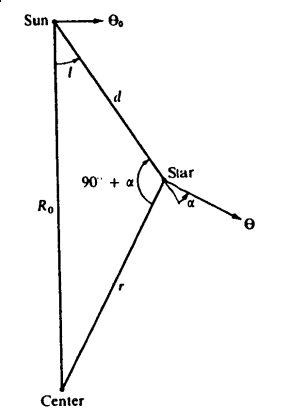
\includegraphics[width=0.3\textwidth]{geom}
  \caption{The relevant geometry of our galaxy. Known constants are the distance from our sun to the center of the galaxy,$R_0 = 8.2 \pm 0.5$, and the velocity of our sun. $\Theta_0 = 223 \pm 17$. The viewing angle $\ell$ is determined by the posiiton of our telescope.}
  \label{geom}
\end{figure}
\end{document}
